\documentclass{article}

\usepackage{listings}
\usepackage{color} %red, green, blue, yellow, cyan, magenta, black, white
\definecolor{mygreen}{RGB}{28,172,0} % color values Red, Green, Blue
\definecolor{mylilas}{RGB}{170,55,241}

\usepackage{graphicx}
\usepackage{subcaption}

\usepackage{float}

\usepackage{geometry}
\geometry{a4paper,margin=2.5cm}
\setlength{\parindent}{0pt} %no indentation between paragraphs
\setlength{\parskip}{4pt} %space between paragraphs

\title{CSSE7014 Distributed Computing \\
Assignment 2 \\
Semester 1, 2017}
\author{Paul Kogel (44644743), Ramdas Ramani (44743767), Andi Nuruljihad (44159069)}

\begin{document}

\maketitle

\pagebreak
\tableofcontents\thispagestyle{plain}

\pagebreak

\section{Introduction}

Fog computing is a new, exciting computing paradigm \cite{bonomi2012fog} that serves as an extension to cloud computing. It allows for tasks traditionally performed at the cloud server to be performed directly by -- or at nodes in closer proximity to -- edge devices.

Cloud computing refers to the usage of remote servers for the purpose of storing, managing, or processing data. Cloud computing has enabled the development and proliferation of advanced services that were previously impossible, like the recognition of voice commands on a smart phone; the phone merely serves as a collector of raw audio data from the user then transmits that data to the cloud where it is processed and the information relevant to the user's query is collected to be sent back to the user.

As the number of devices requesting data from the cloud rises, and the Internet of Things (IoT), the inter-networking of everyday objects via the Internet, continues to expand, cloud services are facing the ever-growing challenge of scaling to accomodate the rising number of objects transmitting and receiving data. This puts a strain on bandwidth as the millions of devices are in a state of constant connection with to the cloud.

Inherent in cloud computing is the problem of latency; data is stored and processed at remote servers in off-site locations that could be anywhere in the world. In addition, the quality of a cloud-based service is highly dependent on the network conditions of a region or area. When you lose your connection to the Internet, you lose the ability to use these services. These are two of the greatest problems faced by developers of smart services that rely on low-latency or real-time response and highly-reliable connections, such as health and emergency services. A delay of even a half-second could pose a safety risk or affect treatment.

Fog computing solves these problems by offloading much of the workload of the cloud server to devices that are closer to the edge \cite{cisco2015fogcomputing}. These devices, or "fog nodes", can be any device with storage and processing power. This means more data is stored and processed locally, reducing the volume of network traffic being sent to and from the cloud, and since more of the data analysis and processing is performed at a location much closer to the user, latency, and subsequently response time, is greatly diminished.

This report will go into detail about the architecture and models of fog computing, common issues in the implementation of fog computing, and real-use applications of the paradigm.

\section{Architectures and Models}
%Compare and contrast different architectures and models with examples to back the arguments.

Fog computing is an emerging cloud paradigm that extends the traditional cloud computing paradigm to the edge of the network to decrease latency and network congestion,enabling the creation of refined and better applications or services. Fog is an edge computing and micro data center (MDC) paradigm for IoTs and wireless sensor networks (WSNs).

Research on fog computing is in its early stages; therefore, no standard architecture is available regarding managing resources in the fog. However some conceptual ones are discussed below.
\subsection{OpenFog Reference Architecture}

The OpenFog RA is driven by a set of core principles called pillars\cite{openfogconsortium2017}.
The pillars represent the key attributes that a system needs to embody the OpenFog definition of a horizontal, system-level architecture that provides the distribution of computing, storage, control, and networking functions closer to the data source (users, things, et al) along the cloud-to-thing continuum\cite{openfogconsortium2017}.
The Pillars are Security, Scalability, Openness, Autonomy, Programmability, Reliability, Availability and Serviceability (RAS), Agility and Hierarchy.

The functional viewpoint of the architecture describes how the OpenFog architectural elements and views are applied to satisfy the stakeholders requirements/concerns on a given scenario. It is however important to note that these change over time. 

The Deployment viewpoint addresses how the fog software and fog systems are deployed in order to satisfy a given scenario. The deployments generally happen in a Hierarchical based model where the number of tiers will be dictated by the scenario requirements\cite{openfogconsortium2017}.
The scenarios might be the amount and type of work required by each tier or the Number of sensors required for the deployment and so on.

The OpenFog RA description is a composite representation of various stakeholder concerns which are referred to as views. The stakeholders and their associated views are identified because they are required to facilitate any successful fog based deployment\cite{openfogconsortium2017}. 

The abstract architecture is viewed from the point of perspectives\cite{openfogconsortium2017} which are namely 
\begin{itemize}
\item Performance - This is a cross cutting concern as it impacts system and deployment scenario. Eg Low Latency
\item Security - Data integrity is a special aspect of security for devices that currently lack adequate security. This includes intentional and unintentional corruption.
\item Manageability - Managing all aspects of fog deployments, which include RAS, DevOps etc. 
\item Data Analysis and Control -  The Autonomy of fog nodes requires localized data analytics coupled with control.
\item IT Business and Cross Fog Applications -  Ability to migrate and properly operate at any level of a fog deployment’s hierarchy.  
\end{itemize}

The views\cite{openfogconsortium2017} described in the OpenFog RA description include 
\begin{itemize}
\item Software View - Represented in the top 3 layers shown in fig below.
\item System View - Represented in the middle Layers shown in fig below.
\item Node View - Represented in the bottom layers shown in fig below.
\end{itemize} 

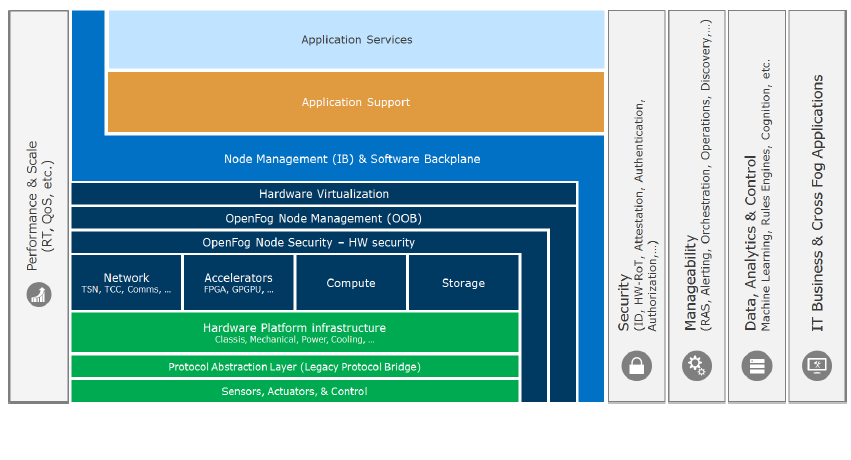
\includegraphics[scale=0.7]{figa.png}

\subsection{OpenFog Deployment Models} 
The models discussed below use a combination of fog and cloud deployment to address various domain scenarios as framed by the layered view of IoT systems.
In real world deployment models, there may be combinations of physical deployments that involve multi-tenants, fog, and cloud deployments owned by one or more entities. 
\subsubsection{Fog Model Independent of the Cloud}
This model is mainly used in cases where cloud cant be used. The reasons might be response time concern, compliance to regulations, security and privacy, and unavailability of a centralised cloud. 
Use Cases include armed forces combat systems, drone operations, some healthcare systems, hospitals, and ATM banking systems.
\subsubsection{Model using Cloud for Business Support}
This model uses cloud for Business Support ( information processing related to decision making).  However the actual Operation-centric information processing is done by fog deployments located close to the infrastructure/process being managed.
Use Cases include commercial building management, commercial solar panel monitoring, and retail.
\subsubsection{Model using Cloud for Business and Operational Support}
This model uses local fog infrastructure for time-sensitive computation, while the cloud is used for the balance of operational and business-related information processing.    
Use Cases include commercial UPS device monitoring, mobile network acceleration, and content delivery networks (CDNs) for Internet acceleration.
\subsubsection{Model using Minimal/no Fog infrastructure}
This model leverages the cloud for the entire process due to the constrained environments in which the deployment of fog infrastructure may not be feasible or economical. However fog nodes that are at device layer may get some monitoring and control functions for safety related control.
Use cases include agriculture, connected cars, and remote weather stations  
\subsection{Gateway based Architecture}
Wangbong lee et.al\cite{lee2016gateway} proposed a Gateway based fog computing architecture that mainly consists of master nodes and slave nodes and manages virtual gateway functions, flows and resources.

A usecase of the architecture proposed below would be WSAN (WIRELESS SENSOR AND ACTUATORS NETWORK).Wireless Sensor and Actuators Network is a group of sensors and actuators linked by wireless medium to perform distributed sensing and actuation tasks. 
The architecture proposed is shown in the figure below.A physical as well as a logical view is shown. The setup included sets of gateway and micro server wherein the gateway and micro server were connected by Ethernet Interface.Interfaces between gateway nodes are wired interfaces and wireless interfaces such as 3G, LTE, and Ethernet\cite{lee2016gateway}.

The slave nodes had functions such as flow management, virtual gateway and resource management and Master nodes had their control functionalities. 

Master node controlled the virtual path of virtual gateway function located in the slave nodes. The Flow management was based on the software defined network such as OpenFlow and virtual function management was provided by a virtualized software middlebox such as ClickOS\cite{lee2016gateway}. 

This architecture provided the WSAN virtualization and the model was event driven. It provided virtual event from networked objects and shared them to various applications.WSN virtualization can help realize the SaaS model through cost efficient utilization of deployed sensors\cite{lee2016gateway}. 

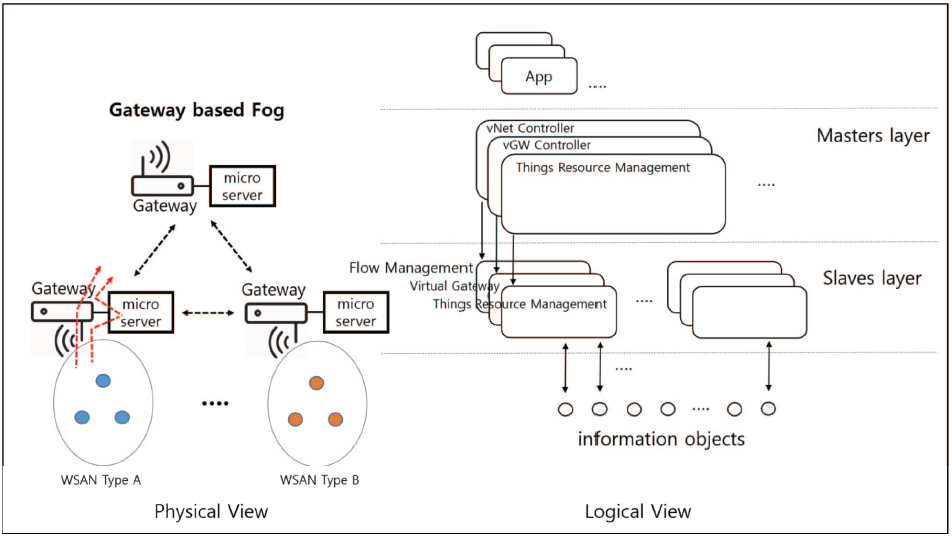
\includegraphics[scale=0.7]{gateway.png}

\subsection{Software-Defined Fog Network Architecture for IoT}
Slavica Tomovic et.al\cite{tomovic2017software} proposed a model of IoT architecture which takes advantage of SDN and Fog computing paradigms.

The architecture involved end devices with multiple wireless communication solutions, SDN controllers, heterogeneous Fog infrastructure (virtualized servers, routers, access points, etc.) and Cloud in the network core\cite{tomovic2017software}.
The fog nodes exposed a set of APIs (Application Programming Interfaces) for application deployment and development, resource management and control. Hierarchical deployment of Fog Architecture was assumed in this case.
Development of IoT applications using hierarchically deployed and heterogeneous Fog resources could be simplified by adopting Mobile Fog programming model\cite{tomovic2017software}.
The same application code is run on various devices of the heterogeneous Fog infrastructure. The application consists of multiple processes that perform different tasks with respect to the device capabilities and position in the network hierarchy. For example, tasks of large-scale video surveillance application may be organized in three levels: motion detection at IP camera, face recognition at edge Fog nodes and aggregation of identities at Cloud server.
In order to achieve service orchestration,logical centralization of orchestration functionality at SDN controller was proposed\cite{tomovic2017software}. 
So, the basic function of the traditional SDN controller was modified to perform
\begin{itemize}
\item Fog Orchestration
\item Speading routing Logic into SDN-enabled network elements
\item Optimally selecting access points for IoT devices.
\end{itemize}  
 
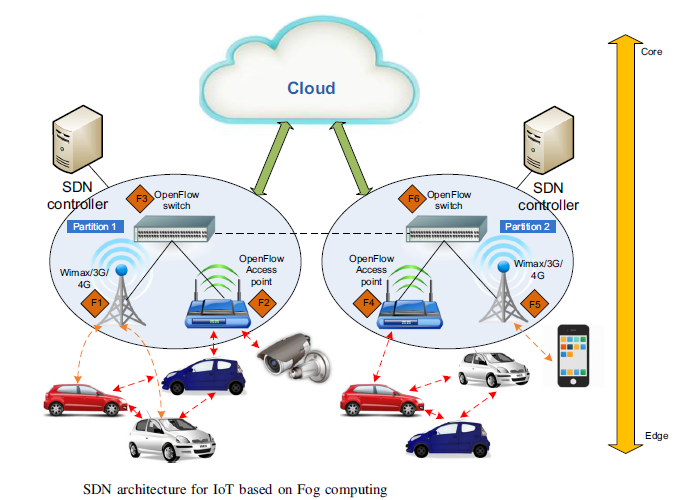
\includegraphics[scale=0.8]{sdn.png}

Use Case of the above proposed architecture would be 
Smart Transportation. With SDN and fog computing, mechanisms for service differentiation and ability to provide real time delivery is met. Beside Fog computing, the presented system model can also exploit benefits of SDN to dynamically assign higher priority to some traffic flows in emergency situations, and hence guarantee low-latency. 


\pagebreak

\section{Common Issues}
% Comments on issue related to communication paradigms, fault tolerance, consistency, reliability, etc.
% Marking criteria: Quality discussion and explanation on relevant issues as required with clear examples. Discussions of potential enhancement to address any performance issues are provided.

Though still an emerging field, previous research, such as Yi et al.'s ``survey on fog computing'' \cite{yi2015survey}, has been able to identify multiple potential issues related to fog computing. In this section, we summarise their main findings, and provide additional discussion and research related to them whenever possible.

To improve clarity, we organise issues around 5 main areas: networking, optimal use of resources, fault tolerance, application development, and security and privacy. Note that we focus purely on technical issues. Business-related aspects, such as implementation of a viable business model, and billing mechanisms, are not covered.

\subsection{Networking}
In order for the fog to function properly, the network has to provide nodes with connectivity, and additional network services, such as routing. The particular nature of the fog, though, makes the implementation of these functions difficult. 

For example, the network has to be highly scalable, providing support for a large number of potential nodes. In addition, it should account for constant topology changes due to node mobility. Ensuring that the system is fully distributed is also an important aspect \cite{yi2015survey}.

Using virtualisation mechanisms, such as SDN, has been deemed as viable solution to these issues \cite{yi2015survey}. In their proposal of a general architecture for the fog, Bonomi et al. \cite{bonomi2014fog} state that the fog should use virtualisation for ``key resources'', including networking. Providing an implementation of SDN for the fog, however, is still an open issue \cite{yi2015survey}. Partly, this appears to be the case because SDN itself does not put ``a high emphasis'' on distribution \cite{peng2016fog}.


\subsection{Optimal resource use}
\label{sub_opt_res_use}

As stated before, the fog is highly heterogeneous. This heterogeneity is greatly reflected by different degrees of resource availability throughout the system. Important resources are storage, computation power and bandwidth. For example, in parts of the system, available bandwidth might be high due to the presence of more powerful network links, while in others, it can be a scare resource.

Naturally, these resources should be ``optimally'' used. However, the actual optimisation goal is highly dependent on the use case: for example, in a real-time application, the main objective is to ensure a small delay. Using more bandwidth or computation power to meet this goal is a valid trade-off. For a computation-heavy application running on a mobile device, in contrast, reducing the amount of computation performed locally on the device might be most important.

In their paper, Yi et al. \cite{yi2015survey} present several strategies that might be used to optimise resource use under different circumstances. 
%
Firstly, they suggest that the adequate placement of data can help optimising bandwidth use. In the previously given example of a real-time application, storing data on nodes that are well-connected to the consumer could significantly reduce delay. This placement, however, has to take the dynamic nature of the fog into account. If a node changes location, for example, data placement on the same node can result in small latencies at one time, but introduce great delays at another time. Even if the location of the consumer does not change, available bandwidth at a link might, e.g. if more nodes are interested in the data.
%
Besides placing data, the authors also suggest to place computation. Using ``computation offloading'', an operation can be partly or fully delegated to a different node in the network. In the aforementioned example of the computation-heavy application, for instance, a more powerful node could perform most of the computation-intense work. Determining which parts of the computation to offload to which nodes, though, can be challenging. As for data placement, this is largely due to the dynamic nature of the fog.
%
Lastly, they present different methods based on the concept of adjusting the network topology. For example, they suggest that effectively choosing the relay nodes for one or multiple endpoints could help reducing delay, while increasing throughput. Again, however, constant changes in the environment, especially the topology, make an implementation challenging.

Focusing less on choosing locations for data and operations, and more on resources actually available at a given node, Aazam and Huh \cite{aazam2015dynamic} present a resource management method that has been developed especially for the dynamic environment of the fog. At its core, their method predicts the resources required by a consumer for the use of a specific service, and uses these predictions to give ``guarantees'' about resource availability. For example, a consumer might get a guarantee of 80\% availability for a particular service, meaning that it will have access to all resources required to run the service for most of the time. Predictions are largely dependent on past consumer behaviour. If the node in the previous example had, for instance, frequently disconnected from the service provider, its resource guarantee would be lower. Basically, this means that if not sufficient resources are available, they would preferably be given to nodes that make better use of them. As it can be easily seen, this makes resource allocation considerably fair.

\subsection{Fault tolerance}
As describe before, the fog mainly uses unreliable wireless network links. In addition, nodes are highly mobile. Being able to ensure availability of services, and provide reliability in general are therefore important aspects.

To improve service availability, Yi et al. \cite{yi2015survey} suggest to adjust the network topology (see section \ref{sub_opt_res_use}). For instance, they present the idea of dividing a network into several clusters, with each cluster centred around a ``rich-resource'' node.

Traditionally, reliability in a distributed system can be provided by the means of techniques such as checkpointing or rescheduling (see \cite{tanebaum2013}). According to Yi et al. \cite{yi2015survey}, though, most of these techniques are unfit for the fog, as they introduce too much delay. They conclude that replication might work, but they expect it to be difficult to implement due to the distributed nature of the system. Additional research on the topic does not seem to exist. Madsen et al. \cite{madsen2013reliability} claim to provide such, but fail to give any actual fog computing-related insights.

%"However, taking a checkpoint is often a costly operation and may have a severe performance penalty." (p. 364)


\subsection{Application Development}
As stated in section XX, the fog is dynamic in regards to network topology, and resource availability. In addition, fog nodes might run on different platforms and system architectures \cite{yi2015survey}. Developing applications that are able to run in this environment, and provide high compatibility, can be expected to be difficult. 

To ease development, Bonomi et al. \cite{bonomi2014fog} propose a ``fog abstraction layer'' that hides the underlying heterogeneity, and provides developers with a ``uniform and programmable interface''. Yi et al. make a similar suggestion by calling for a ``unified interfacing and programming model'' \cite{yi2015survey}.

Due to issues mentioned in the beginning, though, we expect that the implementation of such a layer is challenging.

%TODO: what about cisco?

\subsection{Security and Privacy}
Many applications that have been proposed for fog computing are safety-critical, and/or process sensitive data. For example, in vehicle-to-vehicle communication, an insecure system that allows attackers to remotely control the car could have disastrous consequences. In home automation, users might be worried about giving third parties insights into their daily routine.

%Authentication/access control
Stojmenovic and Wen \cite{stojmenovic2014fog} find that providing authentication throughout the system is one of the ``main security issues'' for fog computing. As an example, they describe a smart meter that is modified by a user, and reports then, due to a lack of proper authentication, false readings. As a possible solution, they suggest encryption at node-level. For this, the meter would encrypt its data, and another node would decrypt it before further forwarding the data. Similarly to this, the OpenFog consortium deems access control (to which it counts authentication) as ``key to building a secure system'' \cite{openfogconsortium2017}. 

%Root of trust
In addition to advocating access control, the consortium's reference architecture for fog computing also defines a hardware component called ``root of trust'' that is ``at the heart of the [...] security of the fog node''. This component is tamper proof, and required to be implemented by every fog node. It provides security by creating a ``chain of trust'', i.e., selecting other components such as hardware, software, or other nodes that it considers trustworthy. If a component is compromised, like the smart meter in the example above, it would not gain trust from the root, and therefore not do any harm.
%stresses the importance of providing ``end-to-end security'' in general. To establish that, it

Though access control and the chain of trust promise to provide a solid foundation to a secure fog system, they are both rather general methods. In order to improve security in a given context, it has been suggested in \cite{openfogconsortium2017} to select additional measures based on the specific use case.

To protect privacy, Yi et al. \cite{yi2015survey} suggest to run ``privacy-preserving'' algorithms before data is transferred from the fog to the cloud. As examples, they mention techniques based on differential privacy and homomorphic encryption. Gerla \cite{gerla2012vehicular} makes an interesting point by stating that moving processing from the cloud to mobile devices alone gives users more control over their data. It can be easily seen, however, that this requires the implementation of adequate control mechanisms. The aforementioned reference architecture \cite{openfogconsortium2017} vaguely describes ``privacy attributes'' that a user can assign to his/her data, suggesting that these might be used to control its use.

\pagebreak

\section{Applications}
%Various examples (across different disciplines) provided with clear arguments why they are relevant.

Fog computing was conceptualized as an extension of the cloud to address services and applications for which the cloud paradigm is not entirely suitable \cite{bessis2014big}. As a relatively new model, the potential applications and likely infrastructure and design challenges for the fog are still being explored. However, there is a wide range of possible uses of a paradigm that enables real-time, low-latency processing, reduces bandwidth costs, with the benefits of improved security and governance. This section will detail some possible applications of fog computing in various fields.

\subsection{Real-time Health Monitoring}
Wireless Body Area Networks (WBAN) is an important technology in healthcare Internet-of-Things (IoT) applications that allows for the unobtrusive monitoring and recording of various vital signs of a patient in real-time. Many health-monitoring systems employ cloud servers for their low cost, processing power, and high storage volume. The primary drawbacks of relying on the cloud paradigm for such a system are the high latency and the volume of data transmitted over the network by such a large number of sensor nodes. For such a system that is highly dependent on accurate, real-time processing of large amounts of data, there is a need for the reduction of transmitted data that still guarantees quality of service (QoS) \cite{gia2015fog}.

Gia et al. \cite{gia2015fog} suggest the ``provision of an extra layer in between a conventional gateway and a remote cloud server''. This added layer, the ``fog layer'', would serve to preprocess data from the various sensor nodes, expediting the response time of vital applications while simultaneously reducing the volume of data transmitted to the cloud.

\subsection{Security and Surveillance}
Surveillance and security camers generate massive volumes of data; a single may create over one terabyte of high-definition video data per day \cite{openfogconsortium2017visualsecurity}. Security decisions must be made rapidly as situations may arise where a delay in response can result in a risk to public safety. The latency and reliability issues inherent in cloud solutions, where such large amounts of security information must be transmitted to a remote location, makes the cloud paradigm an imperfect solution for such a problem.

The Open Fog Consortium claims fog computing may serve as a solution for this scenario \cite{openfogconsortium2017visualsecurity}. The paper recommends the deployment of fog nodes that can be designed to intelligently partition video processing between the various edge devices and the cloud. In contrast to traditional cloud models, this design allows video analytics to be performed at fog nodes that are physically close to the site, reducing latency and allowing for quicker response times in emergency situations. Relevant data can then be sent to the cloud to allow for historical analysis over long periods of time and enable data sharing between multiple locations \cite{openfogconsortium2017visualsecurity} (for example, the sharing of data between airports or multiple locations of a hotel chain).

The addition of an extra layer between the edge and the cloud implies additional security in layers in the process of sending data from edge devices to the cloud. Raw camera data can be analyzed at the fog gateways, where rules may be established to determine which data must be sent to the cloud and which can be stored locally, and video processing can be partitioned intelligently between the cloud, the fog gateway, and the edge devices \cite{openfogconsortium2017visualsecurity}.

\subsection{Smart Cities - Traffic Congestion Management}
Traffic management is an ever-growing challenge faced by major cities where road congestion can be attributed to lost productivity, slower response times from emergency services, and high carbon emissions. Various factors that contribute to traffic congestion simply can not be predicted, such as accidents and weather. In addition, traffic management is a challenge that spans multiple jurisdictions; the development and implementation of potential solutions takes place in isolation within each department, hindering information sharing and integration initiatives \cite{openfogconsortium2017trafficmanagement}.

According to the Open Fog Consortium, proposed cloud solutions in Smart Cities, while suggesting a single cloud that connects these many departments, in reality involve multiple clouds for traffic management \cite{openfogconsortium2017trafficmanagement}. The paper notes that these departments are each responsible for the implementation of their own solutions to the traffic congestion problem for areas under their jurisdiction and, as a result, may potentially work with any number of clouds. This segmented approach, where each piece of the solution is developed and deployed in isolation, can result in the accumulation of redundant data and is an obstacle to data sharing between departments which in turn creates delays in response.

The Open Fog consortium describe a possible fog computing model that might be deployed at the city level \cite{openfogconsortium2017trafficmanagement}. The paper suggests that CCTV, camera, electronic signage, and traffic light data might be  captured by roadside or local fog nodes to be analyzed and used locally and later sent to regional fog nodes where the data may be related to other data from different local nodes. These fog nodes at the regional and city level may be used to share information across individual networks, allowing for all relevant departments to share a single, synchronized picture of road-side conditions as they change. In the future, as manufacturers install fog nodes in their vehicles, each vehicle could potentially function as an edge device that connects with other devices on the road. All of this data in aggregate can be used by municipalities to provide a far more detailed view of traffic conditions, allowing for greater control of road conditions and much quicker response times.

\pagebreak

\renewcommand{\refname}{\section{References}}
\bibliographystyle{ieeetr}
\bibliography{lib}

\end{document}
